%\documentclass[11pt,professionalfonts,hyperref={pdftex,pdfpagemode=none,pdfstartview=FitH}]{beamer}
%\usepackage{times}
\documentclass[11pt,professionalfonts,aspectratio=169]{beamer}
\usefonttheme{serif}
\usepackage{presentation_packages}
\usepackage[version=3]{mhchem}
\DeclareSIUnit\year{yr}
\newcommand{\hilight}[1]{\colorbox{green}{#1}}

\definecolor{mygray}{gray}{0.9}
\definecolor{RoyalBlue}{rgb}{0.25,0.41,0.88}
\def\Emph{\textcolor{RoyalBlue}}

\definecolor{tmp}{rgb}{0.804,0.941,1.0}
\setbeamercolor{numerical}{fg=black,bg=tmp}
\setbeamercolor{exact}{fg=black,bg=red}

\mode<presentation> 
{
    \usetheme[hideothersubsections,width=3.5\baselineskip]{Berkeley}
    \usefonttheme{serif}
    \setbeamercovered{transparent}
    \setbeamerfont{section in sidebar}{size=\scriptsize}
    \setbeamerfont{subsection in sidebar}{size=\tiny}
}

\makeatletter
\beamer@headheight=1.5\baselineskip

\setbeamertemplate{sidebar \beamer@sidebarside}%{sidebar theme}
  {
    \beamer@tempdim=\beamer@sidebarwidth%
    \advance\beamer@tempdim by -6pt%
    \insertverticalnavigation{\beamer@sidebarwidth}%
    \vfill
    \ifx\beamer@sidebarside\beamer@lefttext%
    \else%
      \usebeamercolor{normal text}%
      \llap{\usebeamertemplate***{navigation symbols}\hskip0.1cm}%
      \vskip2pt%
    \fi%
}%

\setbeamertemplate{footline}%{split theme}
{%
  \leavevmode%
  \begin{beamercolorbox}[wd=1\paperwidth,ht=2.5ex,dp=1.125ex,leftskip=.3cm,rightskip=.3cm]{title in head/foot}
%    \usebeamerfont{title in head/foot}\mypaper\hfill \insertframenumber/\inserttotalframenumber
    \usebeamerfont{title in head/foot}\insertshorttitle \hfill \insertframenumber/\inserttotalframenumber
  \end{beamercolorbox}
} 
\setbeamertemplate{blocks}[rounded][shadow=true]
\setbeamertemplate{title page}[default][shadow=true,rounded=true]
\setbeamercolor{box}{fg=black,bg=yellow}
\setbeamertemplate{navigation symbols}{}
\makeatother


\title[Asteroid Reconstruction]{\large\textbf Real Time Adaptive Shape Reconstruction for Asteroid Landing}

\author{\vspace*{-0.3cm}}
   
\institute{
	\footnotesize
	{\normalsize\bf{Shankar Kulumani}}\\
	\vspace*{0.2cm}
  	\textbf{Department of Mechanical \& Aerospace Engineering}\\ \vspace*{0.5cm}
 	\begin{figure} %figure%
       	
\includegraphics[width=0.75\textwidth]{gw_txh_2cs_pos}
  	\end{figure}
}
\date{20180421}

\logo{
\includegraphics[scale=0.2]{figures/gw_atx_2cs_rev.pdf}}

\begin{document}
%=======================================================%

\setcounter{framenumber}{-1}
\begin{frame} %-----------------------------%
  \titlepage
\end{frame}   %-----------------------------%

% !TEX Root = ../presentation.tex

\section{Introduction}

\subsection{Motivation}
\begin{frame}[t]{Why send spacecraft to small bodies?}
    \begin{itemize}
        \item<1-> Some properties only available at the small body
            \begin{itemize}
                \item High fidelity gravitational model
                \item Surface samples or return missions
            \end{itemize}
        \item<2-> Gain experience for future missions
            \begin{itemize}
                \item Weak gravitational field allows for less costly manuevers
                \item Asteroid tours for future deep-space human missions
            \end{itemize}
        \item<3-> Avoiding future impacts
            \begin{itemize}
                \item Local spacecraft can aid in ground based tracking
                \item Mitigation: Gravity tractors, kinetic impactors, solar sails
            \end{itemize}
    \end{itemize}

\end{frame}

\begin{frame}{Asteroid Missions}
\begin{itemize}
    \item Science - insight into the early formation of the solar system
    \item Mining - vast quantities of useful materials
    \item Impact - high risk from hazardous near-Earth asteroids
\end{itemize}    

\begin{center}
    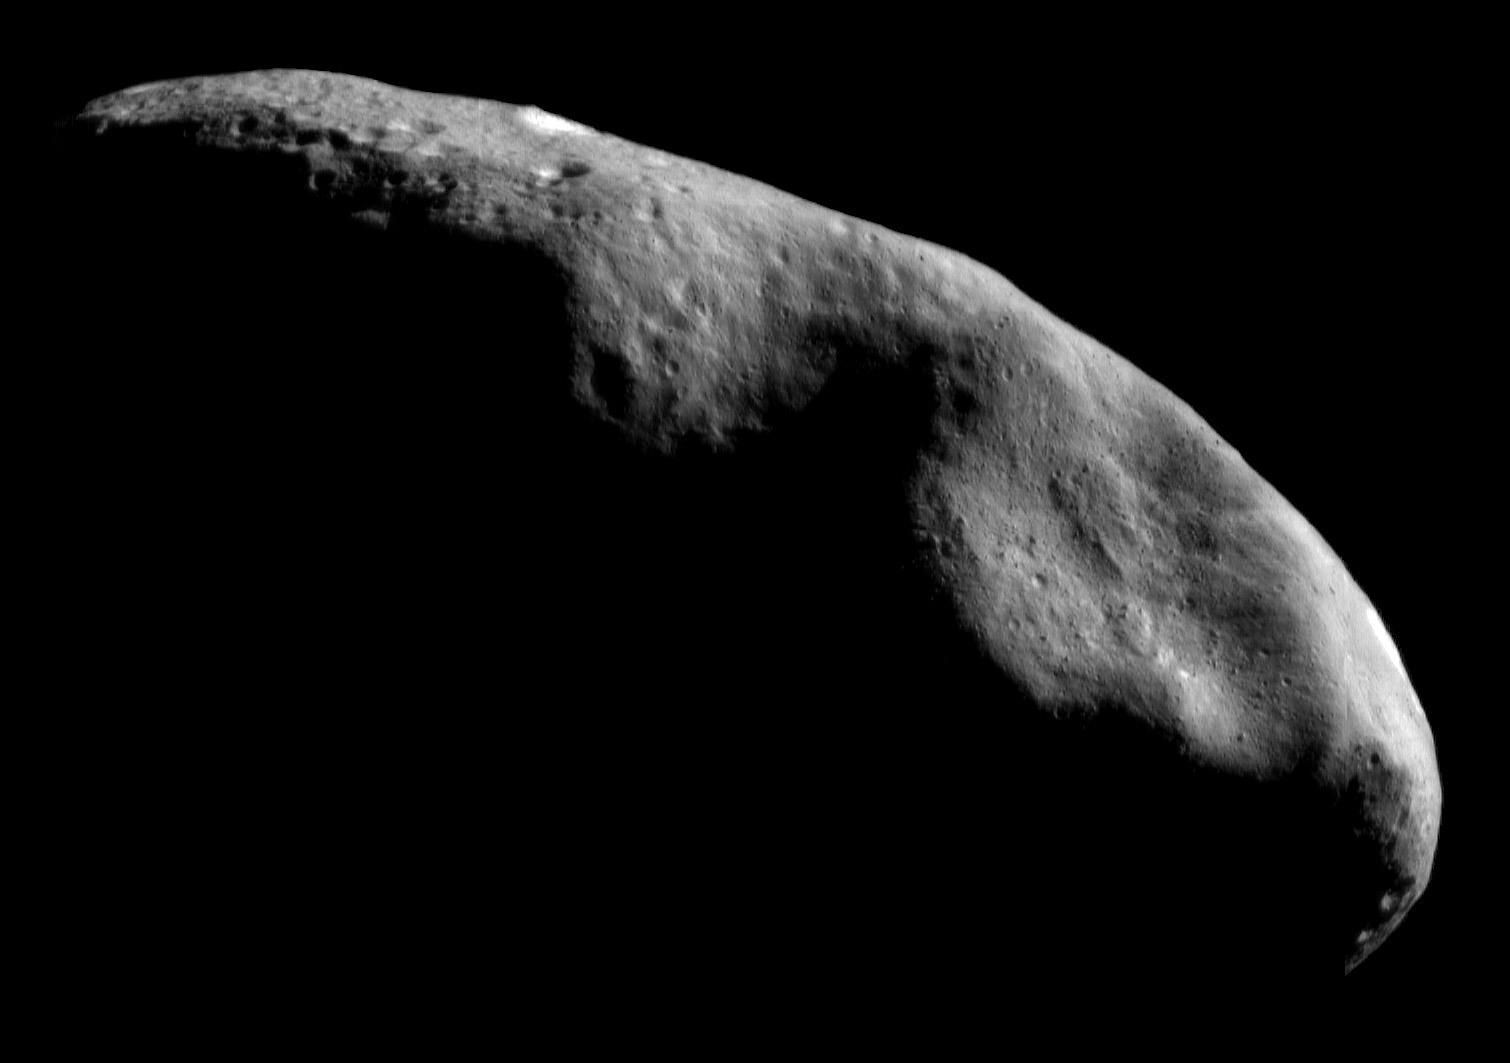
\includegraphics[height=0.5\textheight,width=0.5\textwidth,keepaspectratio]{figures/defense/near_mos_20001203_full.jpg}
    ~
    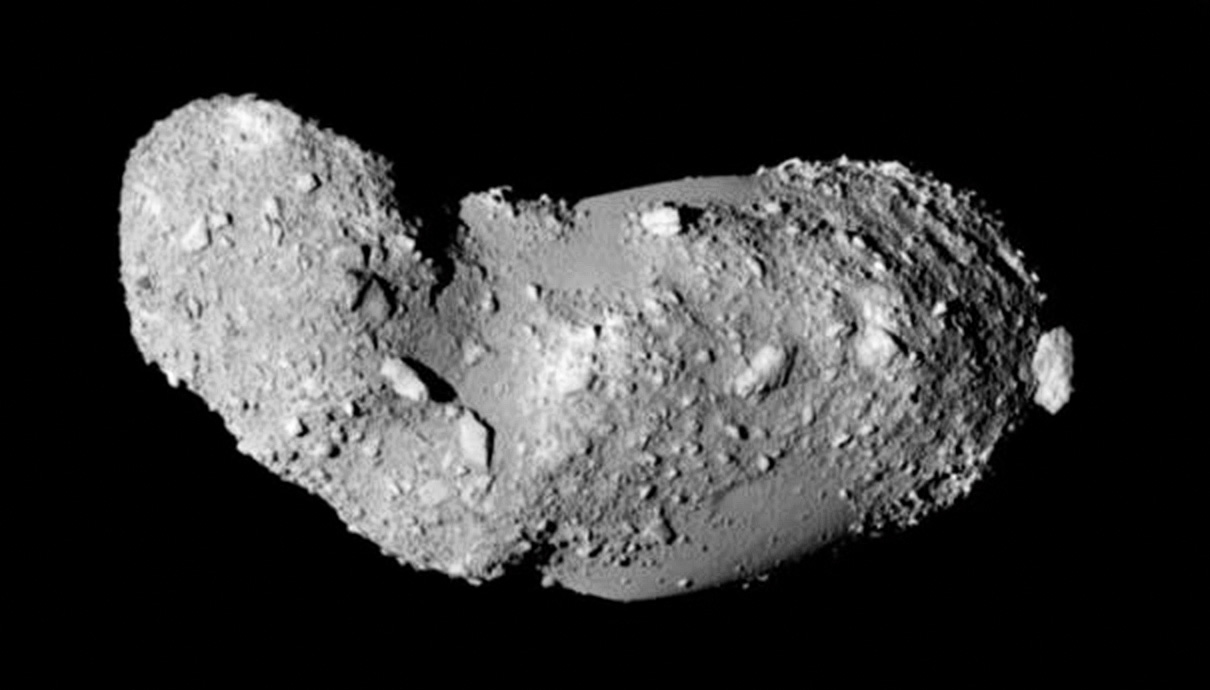
\includegraphics[height=0.5\textheight,width=0.5\textwidth,keepaspectratio]{figures/defense/Itokawa8_hayabusa_1210.jpg}
\end{center}
\end{frame}

\begin{frame}{Asteroid Mining}
    \begin{itemize}
      \item Useful materials can be extracted from asteroids to support:
      \begin{itemize}
          \item Propulsion, construction, life support, agriculture, and precious/strategic metals
      \end{itemize}
      \item Commercialization of near-Earth asteroids is feasible
    \end{itemize}

\pause

\begin{center}
\small
    \begin{tabular}{|l|r|r|}
        \hline 
        Element & Price (\SI{}{\$\per\kilo\gram}) & Sales (\SI{}{\$M\per yr}) \\
        \hline \hline 
        Phosphorous (P) & \num{0.08}  & \num{2167} \\
        Gallium (Ga) & \num{300.00}  & \num{1544} \\
        Germanium (Ge) & \num{745.00} & \num{6145} \\
        \hline \hline 
        Platinum (Pt) & \num{12394.00} & \num{1705} \\
        Gold (Au) & \num{12346.00} & \num{49} \\
        Osmium (Os) & \num{12860.00} & \num{307} \\
        \hline
    \end{tabular}
\end{center}

\end{frame}


\begin{frame}[t]{Problem statement}
    \begin{itemize}
        \item Ground based systems only provide a coarse shape estimate
        \item Spacecraft operations, e.g.\ landing, requires an accurate gravity model
        \item The gravity model accuracy is based on the accuracy of the shape
    \end{itemize}
    \pause
    \begin{center}
    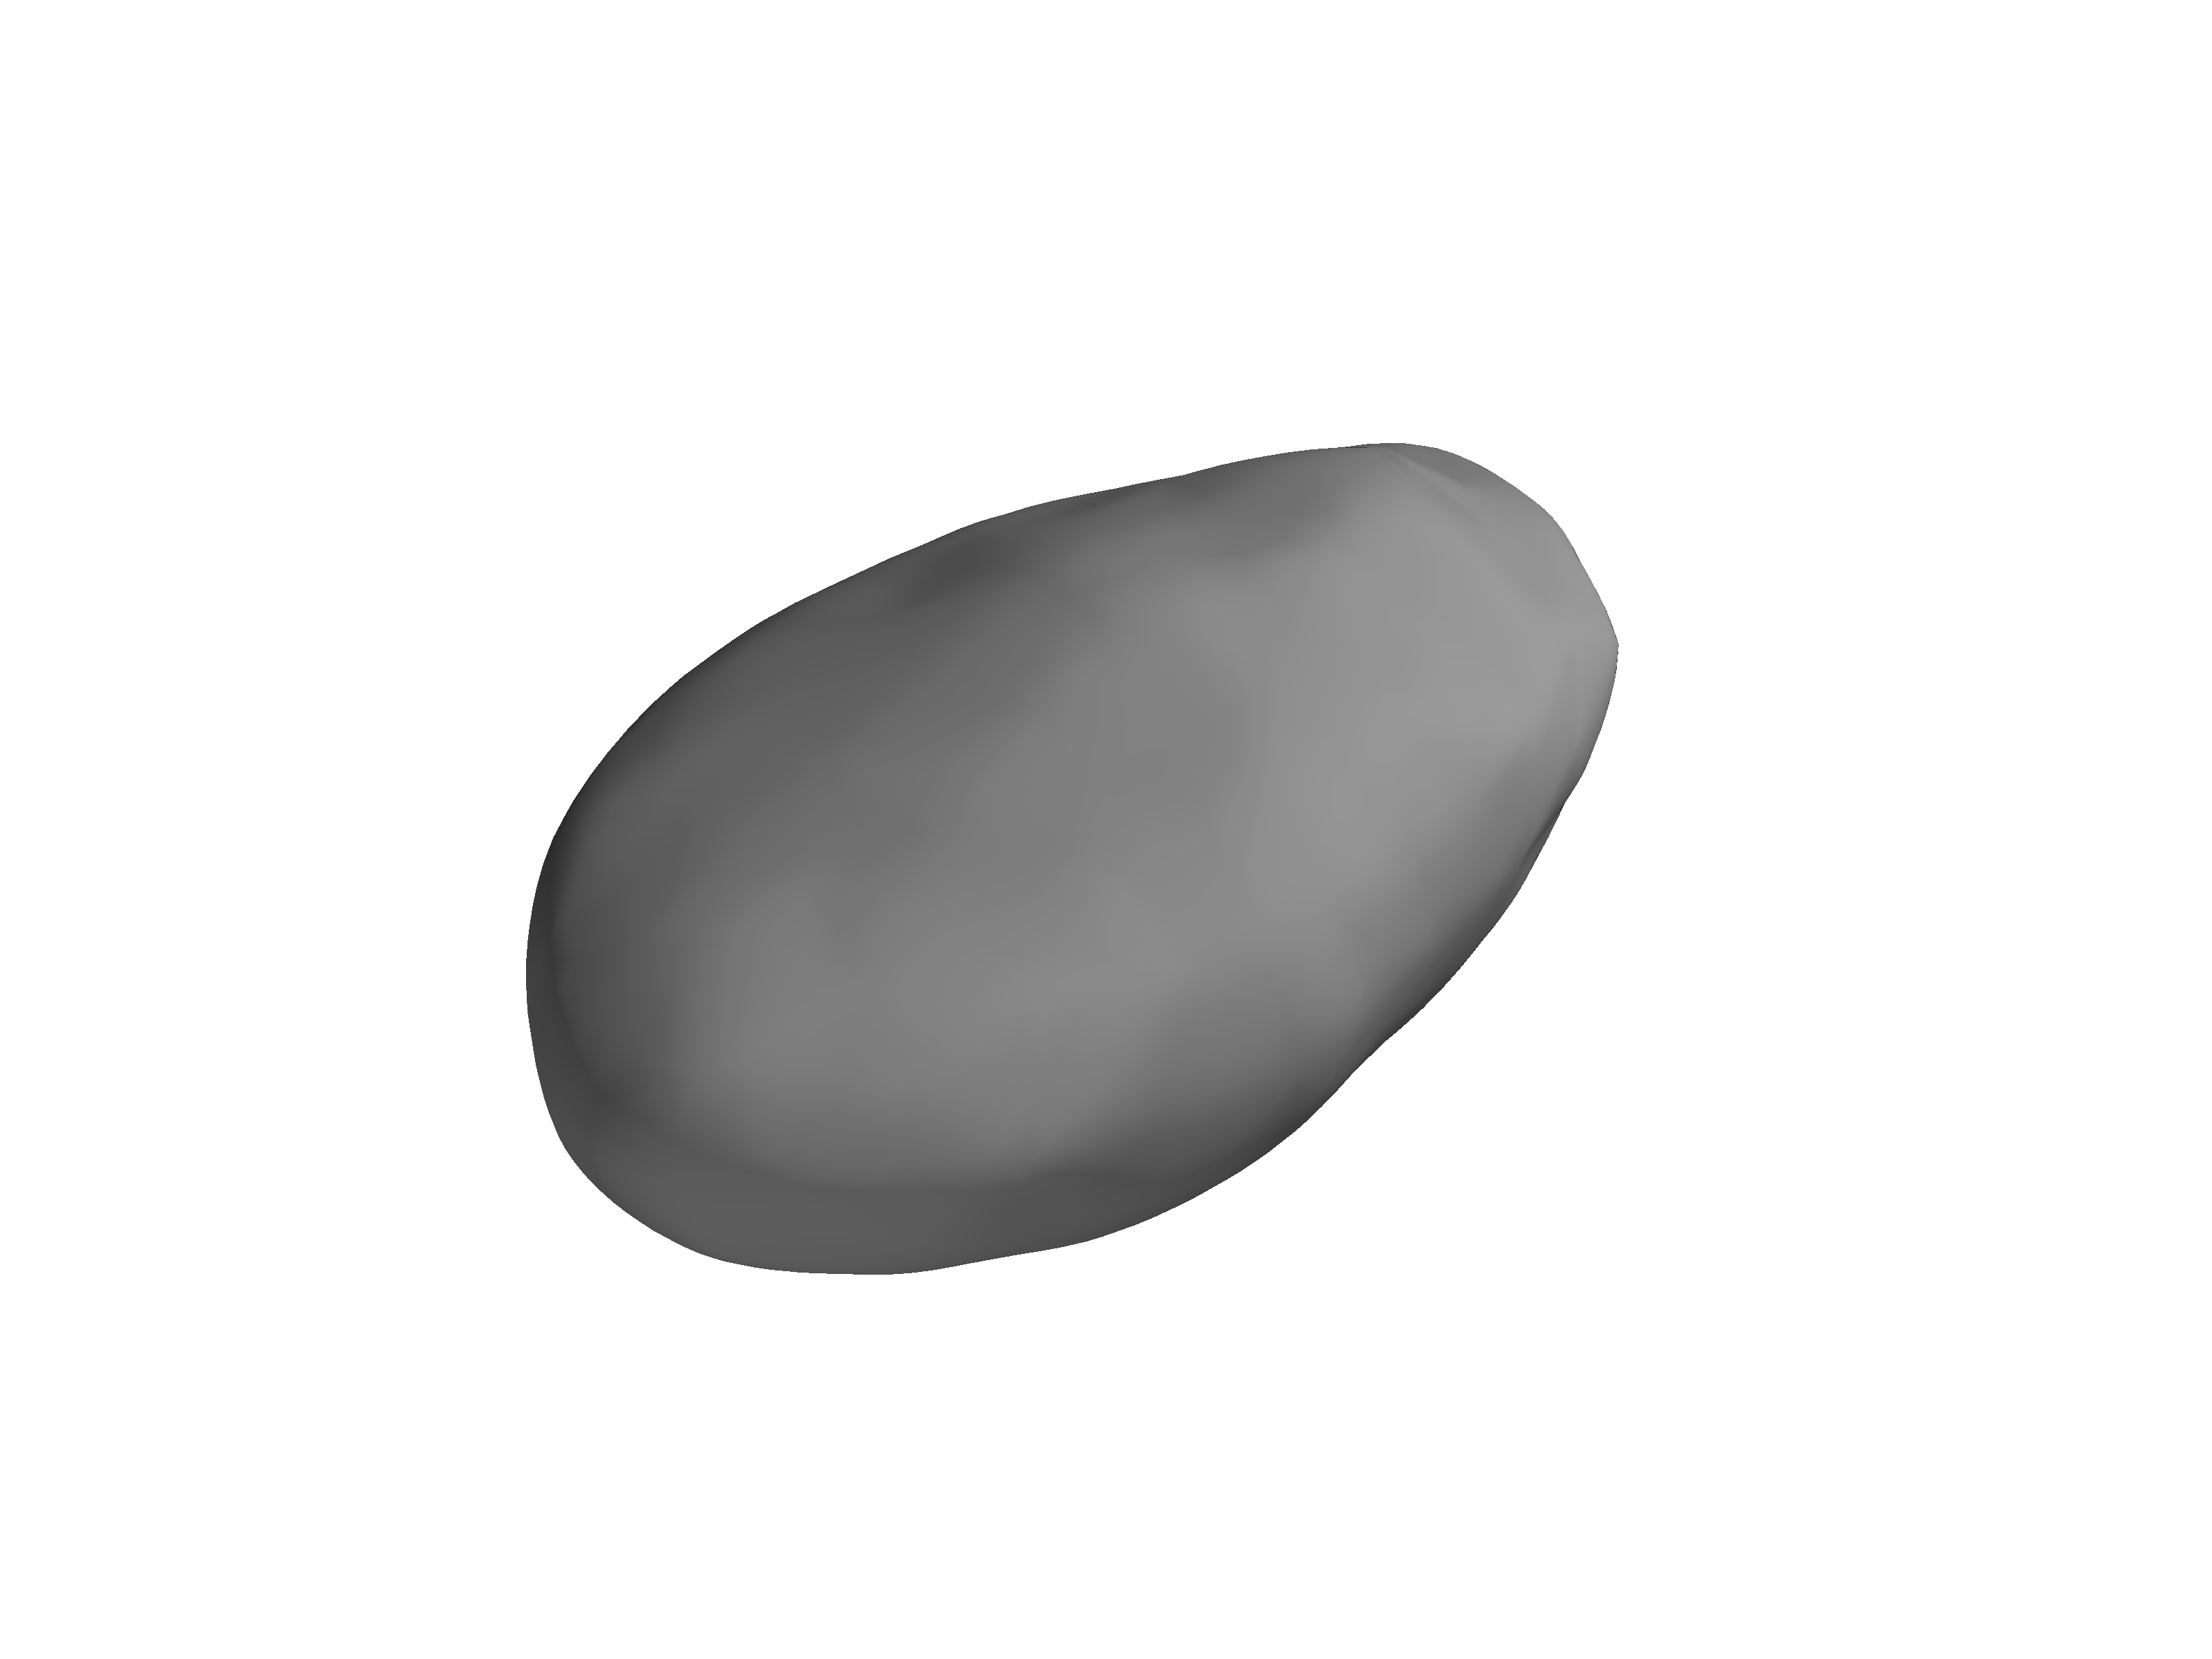
\includegraphics[trim={25cm 15cm 25cm 15cm},clip,width=0.35\textwidth,height=0.5\textheight,keepaspectratio]{figures/mathematical_background/itokawa_radar_isometric.jpg}~
    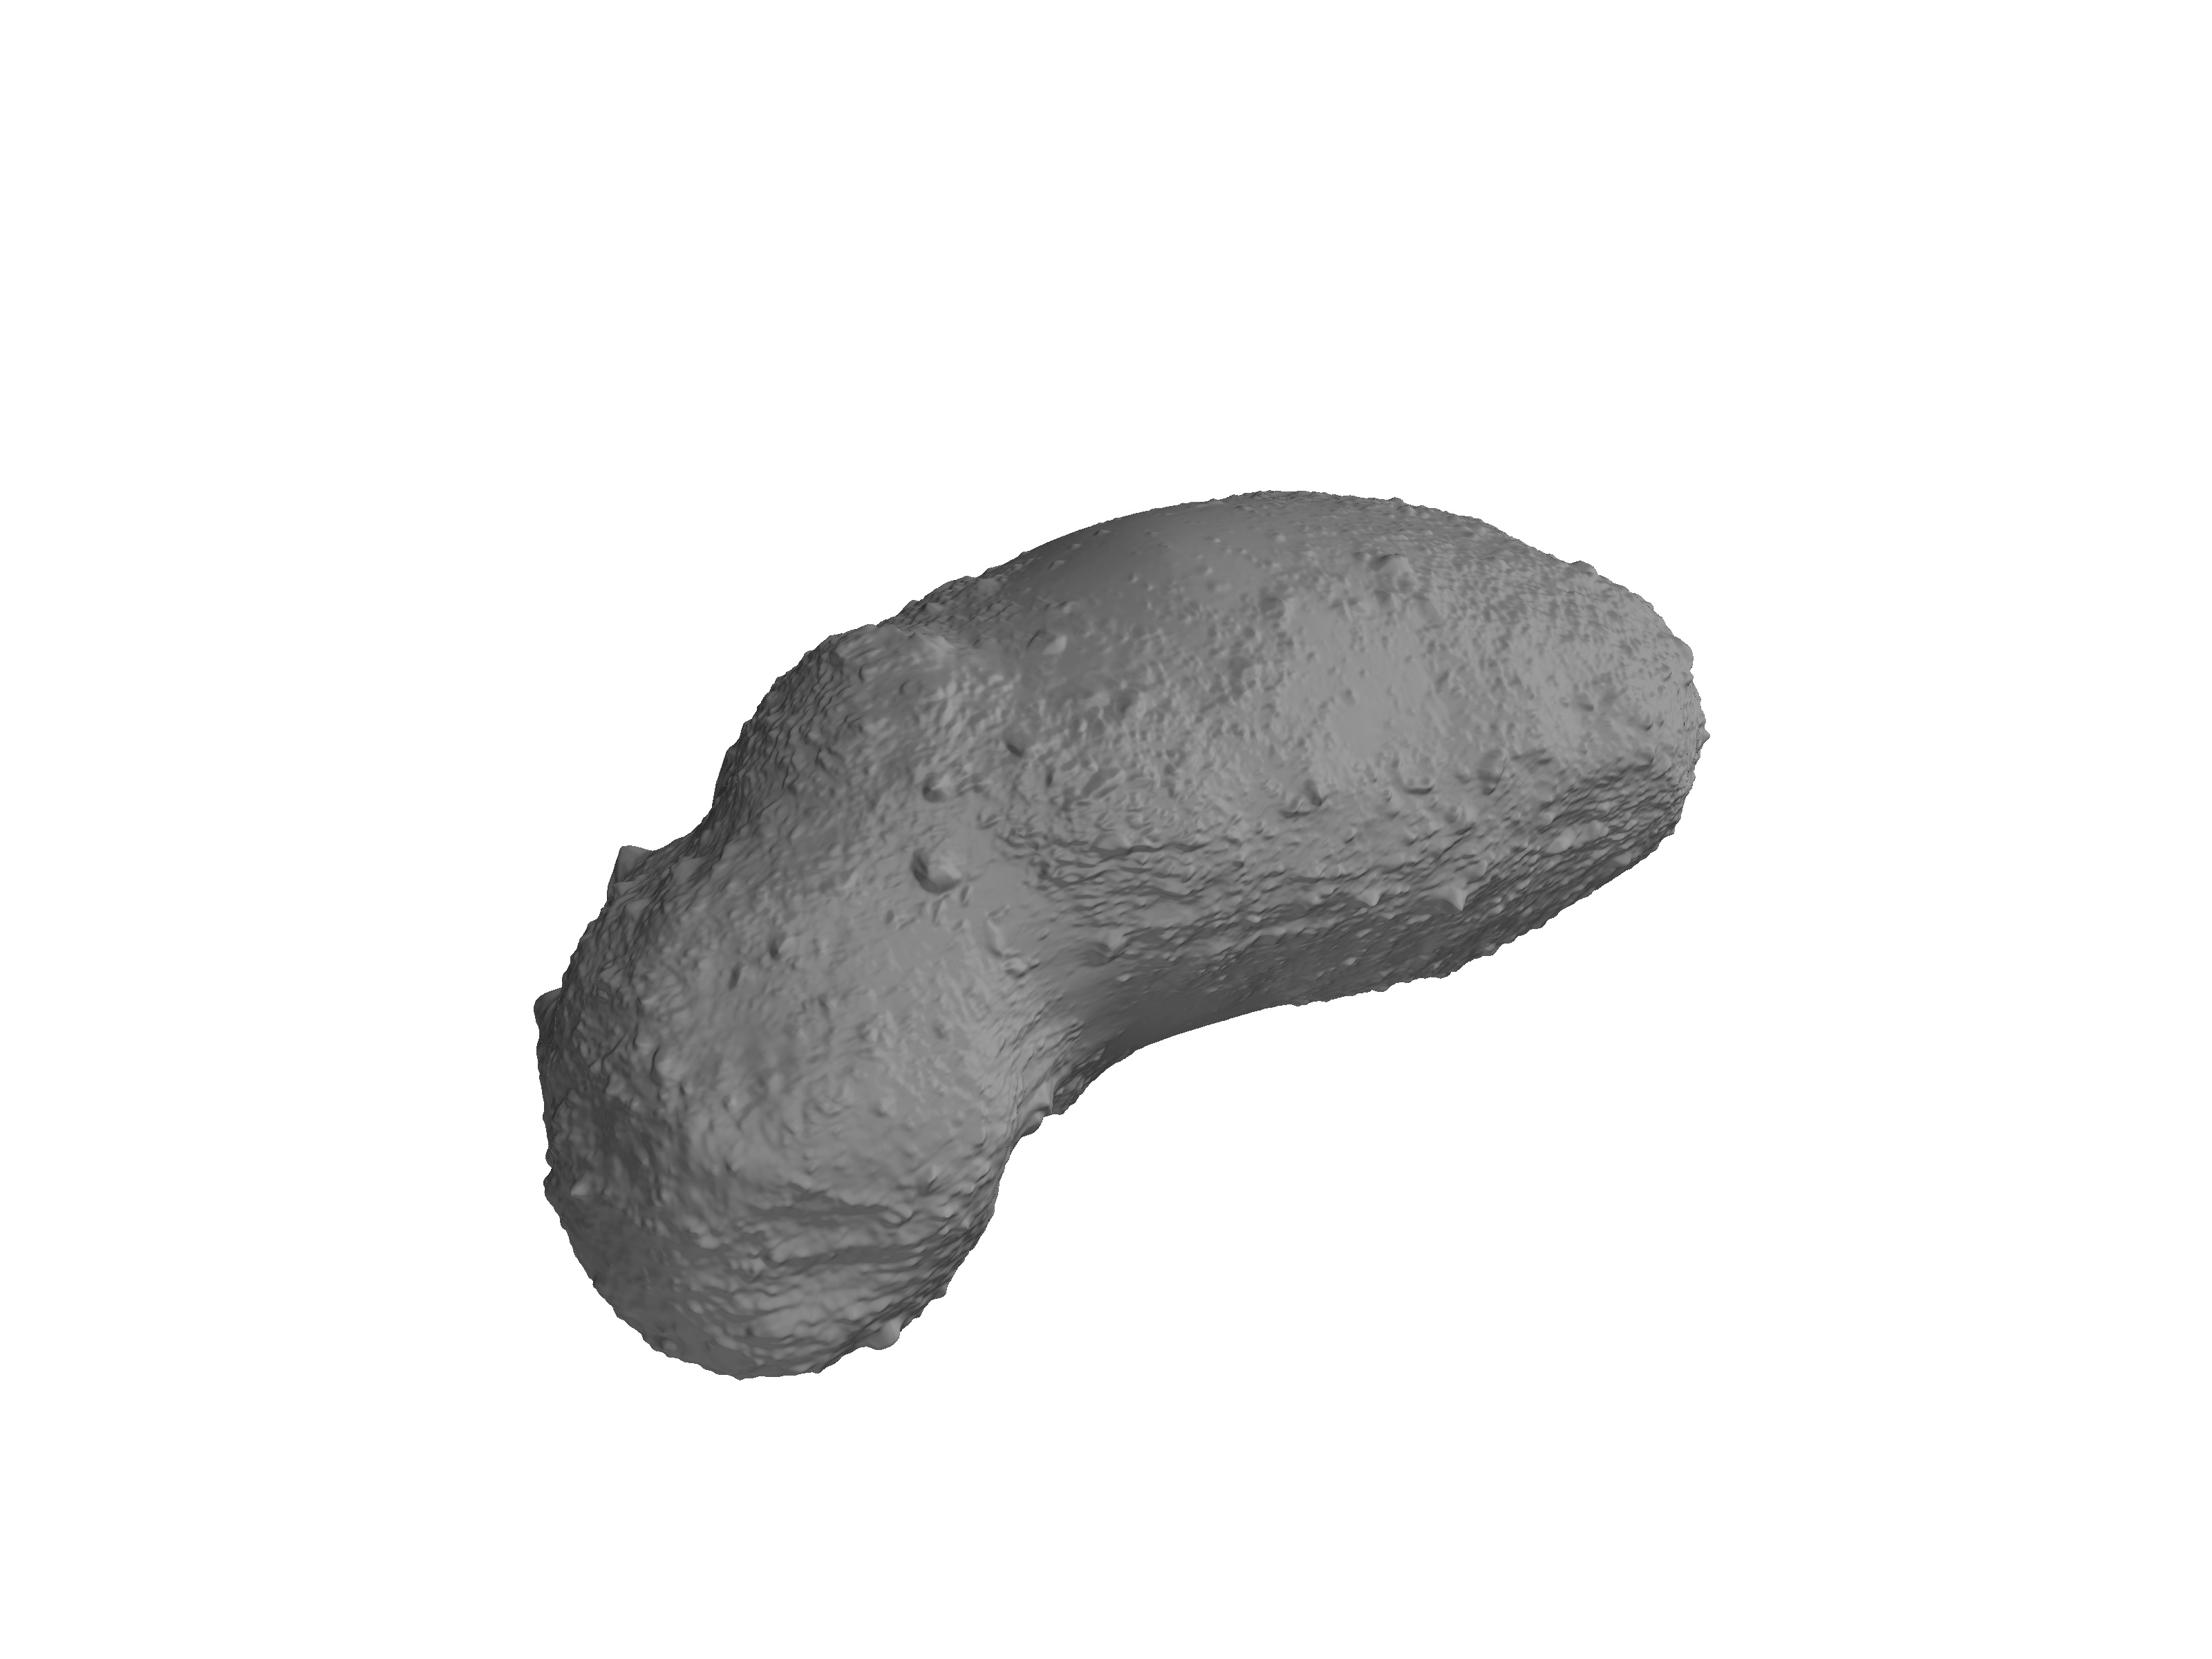
\includegraphics[trim={25cm 12cm 25cm 15cm},clip,width=0.35\textwidth,height=0.5\textheight,keepaspectratio]{figures/mathematical_background/itokawa_isometric.jpg}
    \end{center}
    \begin{block}{}
        \begin{center}
            \begin{enumerate}
                \item Need an accurate shape before arrival
                \item Only in-situ measurements can provide the required detail
            \end{enumerate}
        \end{center}
    \end{block}
    
\end{frame}





\begin{frame}[c]{Thank you}
  \centering
  
  \textbf{\large Flight Dynamics \& Control Lab} \\
  Mechanical \& Aerospace Engineering \\
  School of Engineering \& Applied Science
  
  \begin{figure} %figure%
        
\includegraphics[width=0.75\textwidth]{gw_txh_2cs_pos}
    \end{figure}
  
  \url{https://fdcl.seas.gwu.edu}
\end{frame}
\end{document}

